% figures/geometry/berlinish_composition.tex
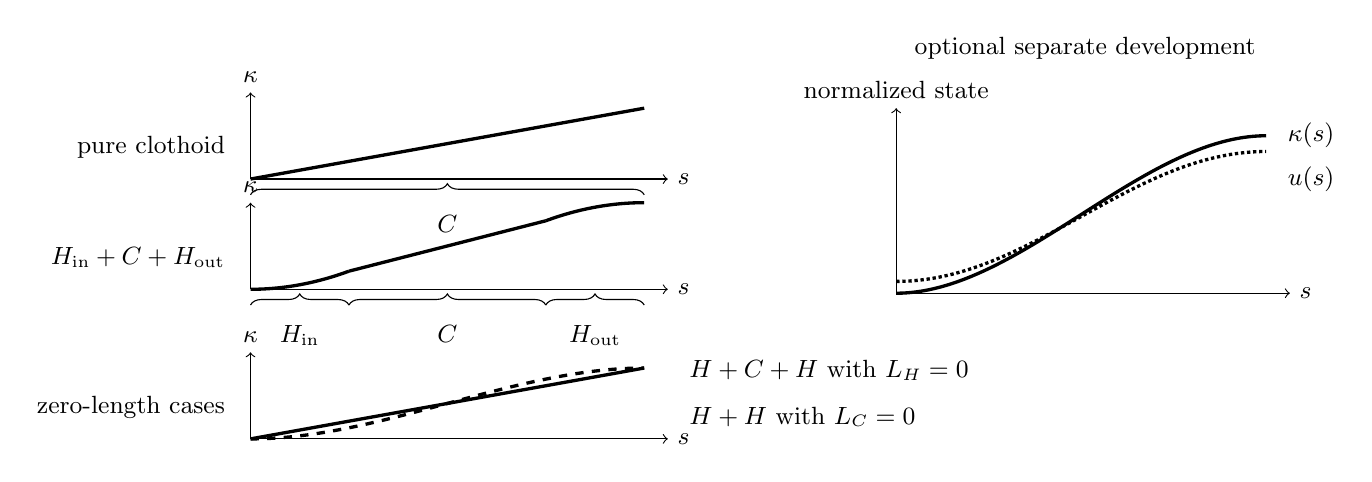
\begin{tikzpicture}[
  x=1cm,y=1cm,
  font=\small,
  axis/.style={->,thin},
  curve/.style={very thick},
  soft/.style={very thick,dashed},
  cant/.style={very thick,densely dotted},
  brace/.style={decorate,decoration={brace,amplitude=4pt}}
]
  % Row 1: pure clothoid
  \node[anchor=east] at (-0.2,3.75) {pure clothoid};
  \draw[axis] (0,3.35) -- (5.3,3.35) node[right] {$s$};
  \draw[axis] (0,3.35) -- (0,4.45) node[above] {$\kappa$};
  \draw[curve] (0,3.35) -- (5,4.25);
  \draw[brace] (0,3.15) -- node[below=4pt] {$C$} (5,3.15);

  % Row 2: full composition
  \node[anchor=east] at (-0.2,2.35) {$H_{\mathrm{in}}+C+H_{\mathrm{out}}$};
  \draw[axis] (0,1.95) -- (5.3,1.95) node[right] {$s$};
  \draw[axis] (0,1.95) -- (0,3.05) node[above] {$\kappa$};
  \draw[curve] plot[smooth,domain=0:1.25,samples=30] (\x,{1.95+0.23*(\x/1.25)^2});
  \draw[curve] (1.25,2.18) -- (3.75,2.82);
  \draw[curve] plot[smooth,domain=3.75:5,samples=30] (\x,{3.05-0.23*((5-\x)/1.25)^2});
  \draw[brace] (0,1.75) -- node[below=4pt] {$H_{\mathrm{in}}$} (1.25,1.75);
  \draw[brace] (1.25,1.75) -- node[below=4pt] {$C$} (3.75,1.75);
  \draw[brace] (3.75,1.75) -- node[below=4pt] {$H_{\mathrm{out}}$} (5,1.75);

  % Row 3: zero-length cases
  \node[anchor=east] at (-0.2,0.45) {zero-length cases};
  \draw[axis] (0,0.05) -- (5.3,0.05) node[right] {$s$};
  \draw[axis] (0,0.05) -- (0,1.15) node[above] {$\kappa$};
  \draw[soft] plot[smooth,domain=0:5,samples=60] (\x,{0.05+0.9*(3*(\x/5)^2-2*(\x/5)^3)});
  \draw[curve] (0,0.05) -- (5,0.95);
  \node[anchor=west] at (5.45,0.92) {$H+C+H$ with $L_H=0$};
  \node[anchor=west] at (5.45,0.33) {$H+H$ with $L_C=0$};

  % Right lower inset: separated kappa and cant
  \begin{scope}[shift={(8.2,1.9)}]
    \node[anchor=south] at (2.4,2.85) {optional separate development};
    \draw[axis] (0,0) -- (5.0,0) node[right] {$s$};
    \draw[axis] (0,0) -- (0,2.35) node[above] {normalized state};
    \draw[curve] plot[smooth,domain=0:4.7,samples=60] (\x,{2.0*(3*(\x/4.7)^2-2*(\x/4.7)^3)});
    \draw[cant] plot[smooth,domain=0:4.7,samples=60] (\x,{0.15+1.65*(0.5-0.5*cos(180*\x/4.7))});
    \node[anchor=west] at (4.85,2.0) {$\kappa(s)$};
    \node[anchor=west] at (4.85,1.45) {$u(s)$};
  \end{scope}
\end{tikzpicture}
